\documentclass[]{article}

% Imported Packages
%------------------------------------------------------------------------------
\usepackage{amssymb}
\usepackage{amstext}
\usepackage{amsthm}
\usepackage{amsmath}
\usepackage{enumerate}
\usepackage{fancyhdr}
\usepackage[margin=1in]{geometry}
\usepackage{graphicx}
\usepackage{extarrows}
\usepackage{setspace}
\usepackage{xcolor}
\usepackage{grffile}
\usepackage[normalem]{ulem}
\usepackage{textcomp}

%------------------------------------------------------------------------------

% Header and Footer
%------------------------------------------------------------------------------
\pagestyle{plain}  
\renewcommand\headrulewidth{0.4pt}                                      
\renewcommand\footrulewidth{0.4pt}                                    
%------------------------------------------------------------------------------

% Title Details
%------------------------------------------------------------------------------
\title{Deliverable \#1 - Software Requirements Specification \\
	SE 3A04: Software Design II -- Large System Design}
\author{Chen, Arthur \and Campbell, Christopher \and Endrizzi, Johnny \\ 
\and Coovert, Mitchell \and Gill, Surinder \and Dhadda, Terin}
\date{February 8, 2016}                               
%------------------------------------------------------------------------------

% Document
%------------------------------------------------------------------------------
\begin{document}

\maketitle	
\newpage
\tableofcontents
\listoftables
\newpage

% Begin Section
\section{Introduction}
\label{sec:introduction}

The following section provides an overview of the entire software requirements specifications document.

\subsection{Purpose}
\label{sub:purpose}
% Begin SubSection
The purpose this document is to outline the requirements for the \textcolor{red}{"BEER'D"} application. This program will be developed as a mobile android application and will be available on the Google Play Store. This document is intended for the developers of the application, Professor Ridha Khedri, teaching assistants for SE 3A04, and any other software engineers or students interested in this project.
% End SubSection

\subsection{Scope}
\label{sub:scope}
% Begin SubSection
The software product to be produced is known as the \textcolor{red}{"BEER'D"} mobile application. This application will allow a user to identify a certain type of beer. This will be accomplished by three experts on the colour of beer, taste of beer, and type of beer, who will form their best choice as to what kind of beer the user describes when selecting some predefined inputs. The application will display these results, display a map of nearby LCBO's and Beer Store's according to the user's current location, as well as some social media sharing features.
% End SubSection

\subsection{Definitions, Acronyms, and Abbreviations}
\label{sub:definitions_acronyms_and_abbreviations}
% Begin SubSection
	\textcolor{red}{N/A}
% End SubSection

\subsection{{References}}
\label{sub:references}
% Begin SubSection
\begin{enumerate}[a)]
	\item \underline{Beer Buddy} app description on \underline{Google Play}  \\
https://play.google.com/store/apps/details?id=com.s2it.beerbuddy\&hl=en
	\item \underline{Untappd} app description on \underline{Google Play} \\
https://play.google.com/store/apps/details?id=com.untappdllc.app\&hl=en
	\\
	
\end{enumerate}
% End SubSection

\subsection{{Overview}}
\label{sub:overview}
% Begin SubSection
\begin{enumerate}[a)]
	\item  The rest of the document will outline general characteristics of the product, and the kind of environment it will be released it. What the product can do and is limited to will be explained more thoroughly as well as a complete description of its functional and non-functional requirements.
	\item Section 2 will describe the more general aspects of the product such as its relation with related products, as well as other systems. It will describe a summary of its functions and its interaction with the user as well constraints, assumptions, and potential requirements for future versions of the product. Section 3 and 4 will have a more extensive statement about the product's functional and non-functional requirements.
\end{enumerate}
% End SubSection

% End Section

\section{Overall Description}
\label{sec:overall_description}
% Begin Section

"What is this Beer?" provides users who are of legal age to purchase alcohol to identify a beer reflective of their preferences and provide them with a method of locating a place that supplies such beer. Locations are specific to \underline{LCBO} and \underline{Beer Store} and are powered by Google Maps API. The application should be usable by anybody with general knowledge of mobile technology. \\


\subsection{Product Perspective}
\label{sub:product_perspective}
% Begin SubSection
\begin{enumerate}[a)]
	\item There are other applications similar to "What is this Beer?" called "Untappd" and "Beer Buddy." Untappd allows the user to find nearby beers and bars and features based around that idea while Beer Buddy allows the user to find out more about a certain beer by UPC code. This application combines the most practical aspects of these applications such as outputting beer stores and beer information via search bar. 
	\item This product is completely separate from the applications mentioned above and is a standalone product.
	\item The product uses interfaces from systems such as Google Maps and LCBO in order to enable the functionality of the location feature and output beer information respectively. It also connects to social media networks such as Facebook, Twitter, and Instagram in order to share a message about the beer picked.
	\item 

		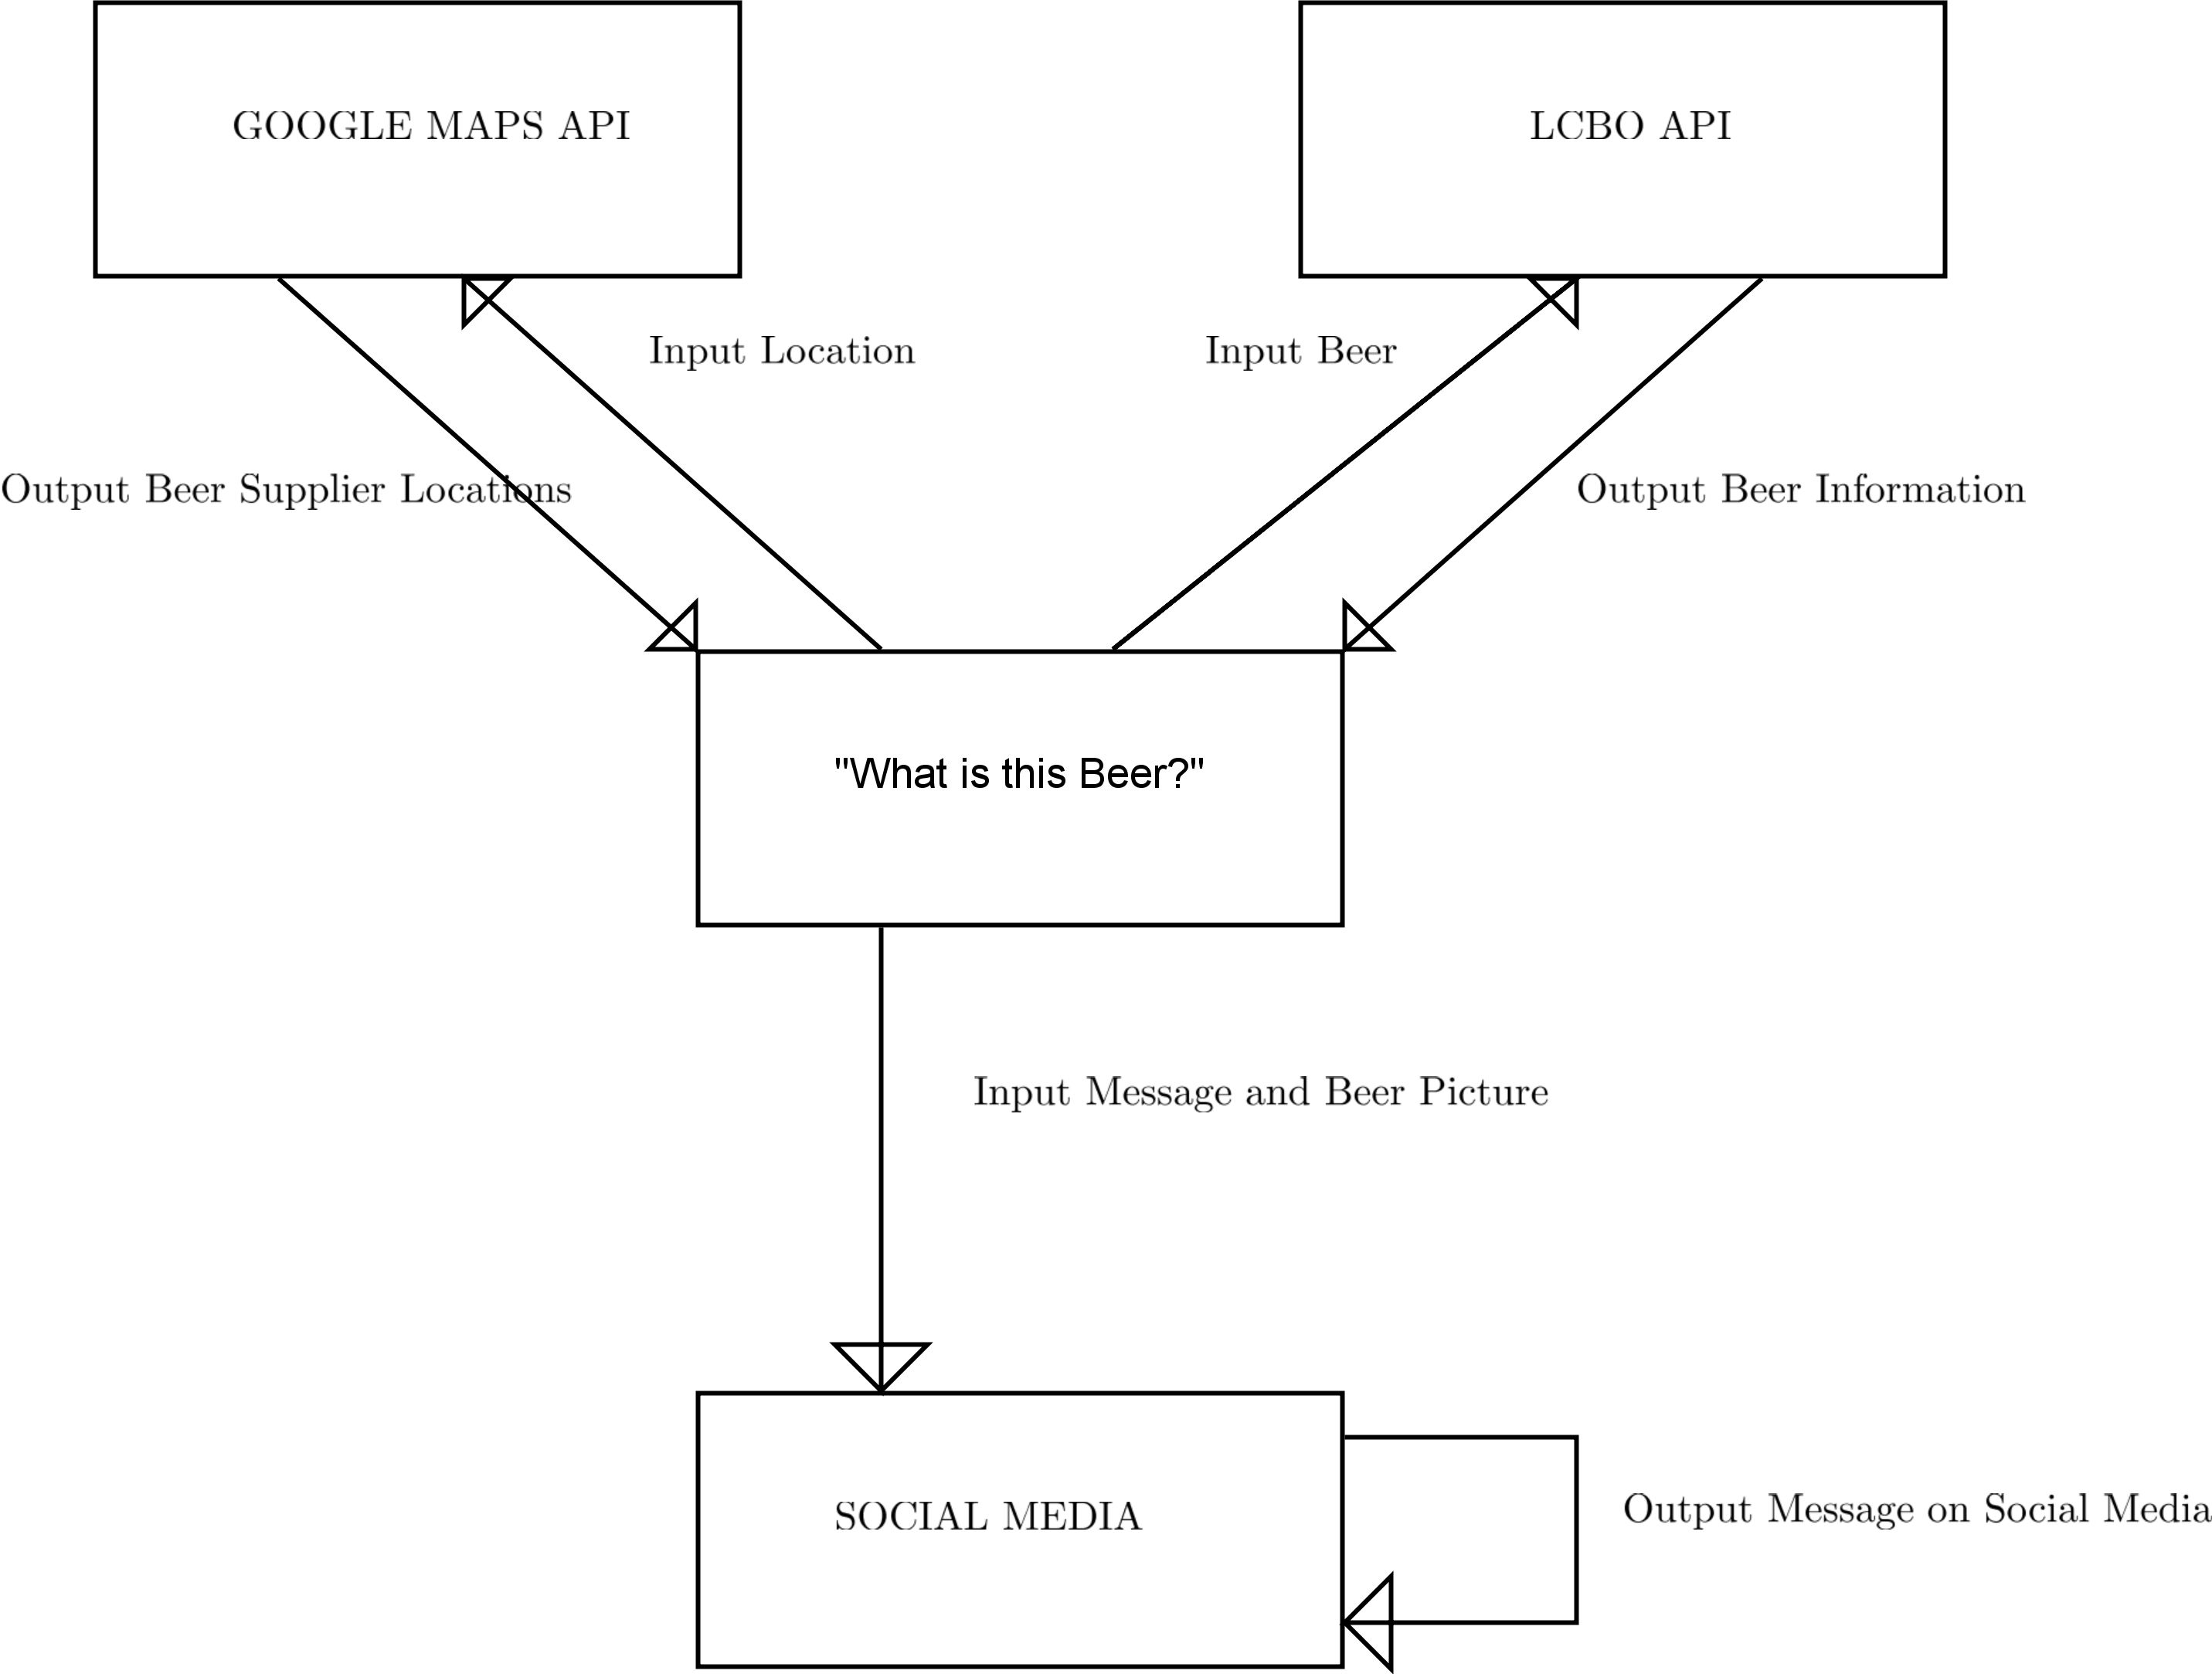
\includegraphics[scale=0.1]{Block Diagram/Block Diagram.jpg}

	
\end{enumerate}
% End SubSection

\subsection{Product Functions}
\label{sub:product_functions}
% Begin SubSection

The software should be able to:
\begin{enumerate}[a)]

\item Search for beers with particular attributes
\item Output beer information of selected beer
\item Locate closest locations to obtain selected beer
\item Share the beer information on social media 

	
\end{enumerate}
% End SubSection

\subsection{User Characteristics}
\label{sub:user_characteristics}
% Begin SubSection
\begin{enumerate}

	\item The User will need a basic knowledge of smartphone use: know where the Playstore is, know how to download applications off of the playstore and follow instructions in the application.
	\item The User also needs to have enough knowledge of beer to identify the taste and type desired.

\end{enumerate}
% End SubSection

\subsection{Constraints}
\label{sub:constraints}
% Begin SubSection
\begin{enumerate}

	\item The application can only search based on specific categories of keywords.
	\item Location functionality only works if location is enabled by the client.
	\item The types of beer offered at local store locations will vary and will limit the amount of information the application is able to output.
	
\end{enumerate}
% End SubSection

\subsection{Assumptions and Dependencies}
\label{sub:assumptions_and_dependencies}
% Begin SubSection
\begin{enumerate}

\item The application depends on information provided by the beer API used such as beer brand, beer taste, cost, etc.
\item The application requires a desired input to be predicted by the application.

\end{enumerate}
% End SubSection

\subsection{Apportioning of Requirements}
\label{sub:apportioning_of_requirements}
% Begin SubSection
\begin{enumerate}
	\item The addition of wines, sprites and other beverages can be added in future version.
	\item Other experts to assist the user in finding the desired beer may also be added.
\end{enumerate}
% End SubSection

% End Section

% Begin Section
\section{Functional Requirements}
\label{sec:functional_requirements}
The following section contains the details about all of the functional requirements about the system. The requirements are split up by viewpoints, and then again by business events, before they go into detail about the functions of the system.\\ 


\begin{enumerate}[{VP}1.]
	\item User
	
	\begin{enumerate}[{BE1}.1]
		
		\item User wants to request information about a beer
		\begin{enumerate}
			\item The system shall display an input screen for the user, where the user will select from a list of predefined words for three separate categories.
			\item The system will have the experts (each corresponding to one category) use the input provided by the user to predict what kind of beer the user may be describing.
			\item The system will create a forum screen which will contain a map of LCBO\textquotesingle s and Beer Store\textquotesingle s that are located within a 50km radius to the user\textquotesingle s current location that offer each type of chosen beer by the experts.
			\item \textcolor{red}{Below the map, there will be three forms of selection: a selection for Facebook, Twitter, and Instagram. If the user has their accounts synced to the system and they chooses one of these selections, the system shall create a message (less than 140 characters) and a picture (of one of the beers chosen by the experts) to share to the corresponding social media account.}
			
		\end{enumerate}
		
		\item User wants to review search history
		\begin{enumerate}
			\item The user must be able to review previous inputs for their searches.
			\item The system must hold data on previous searched entries in memory.
		\end{enumerate}
		
		\item User wants to share beer results
		\begin{enumerate}
			\item The system must display an error if unable to connect to a social media outlet.
			\item The system if successful, must post the results of the user search on user controlled social media outlet(s).
		\end{enumerate}
		
		\item User wants to access general information 
		\begin{enumerate}
			\item The system must display an about screen containing information about beers.
		\end{enumerate}
		
		\item User wants to sync social media accounts 
		\begin{enumerate}
			\item The system must be allow to login to a social media account.
			\item The system must display an error if unable to to connect to a social media connect.
			\item The system must allow a success message once connected to a social media account.
			\item The system must encrypt login credentials when connecting to a social media account.
		\end{enumerate}
		
		
		
	\end{enumerate}
	
	\item Developer
	
	\begin{enumerate}[{BE2}.1]
		\item Developer updates the API(s).
		\begin{enumerate}
			\item The system must be able to request and send information to the desired API(s).
			\item The system shall update it's beer selection based on the data provided in the API(s).
		\end{enumerate}
		
		\item Developer wants to add/remove or change an expert.
		\begin{enumerate}
			\item The system must be able to support addition or removal of an expert as requested.
			\item The system must be able to support a swap or change of an expert.
		\end{enumerate}
		
		\item {Ratings and Feedback are given to the Application }
		\begin{enumerate}
			\item The system shall prompt user to enter for a rating out of 5 after the service is used. 
			\item The system shall send these results to the \underline{Play Store} when there is a valid internet connection.
		\end{enumerate}
		
	\end{enumerate}
	
	
\end{enumerate}

% End Section

\section{Non-Functional Requirements}
\label{sec:non-functional_requirements}
% Begin Section
\subsection{Look and Feel Requirements}
\label{sub:look_and_feel_requirements}
% Begin SubSection

\subsubsection{Appearance Requirements}
\label{ssub:appearance_requirements}
% Begin SubSubSection
\begin{enumerate}[{LF}1. ]
	\item \textcolor{red}{Each menu shall be clearly labeled.}
\end{enumerate}
% End SubSubSection

\subsubsection{Style Requirements}
\label{ssub:style_requirements}
% Begin SubSubSection
\begin{enumerate}[{LF}1. ]
	\item \textcolor{red}{\emph{N/A}}
\end{enumerate}
% End SubSubSection

% End SubSection

\subsection{Usability and Humanity Requirements}
\label{sub:usability_and_humanity_requirements}
% Begin SubSection

\subsubsection{Ease of Use Requirements}
\label{ssub:ease_of_use_requirements}
% Begin SubSubSection
\begin{enumerate}[{UH}1. ]
	\item The application shall \textcolor{red}{be available} for a person aged 19+ in able condition to understand and use all of its features.
\end{enumerate}
% End SubSubSection

\subsubsection{Personalization and Internationalization Requirements}
\label{ssub:personalization_and_internationalization_requirements}
% Begin SubSubSection
\begin{enumerate}[{UH}1. ]
	\item The application shall \textcolor{red}{retain the users previous location, and search settings.}
\end{enumerate}
% End SubSubSection

\subsubsection{Learning Requirements}
\label{ssub:learning_requirements}
% Begin SubSubSection
\begin{enumerate}[{UH}1. ]
	\item The application shall be able to be used by members of the public with no previous training.
\end{enumerate}
% End SubSubSection

\subsubsection{Understandability and Politeness Requirements}
\label{ssub:understandability_and_politeness_requirements}
% Begin SubSubSection
\begin{enumerate}[{UH}1. ]
	\item "What is this Beer" shall use words and symbols understandable by its user community.
\end{enumerate}
% End SubSubSection

\subsubsection{Accessibility Requirements}
\label{ssub:accessibility_requirements}
% Begin SubSubSection
\begin{enumerate}[{UH}1. ]
	\item \textcolor{red}{\emph{N/A}}
\end{enumerate}
% End SubSubSection

% End SubSection

\subsection{Performance Requirements}
\label{sub:performance_requirements}
% Begin SubSection

\subsubsection{Speed and Latency Requirements}
\label{ssub:speed_and_latency_requirements}
% Begin SubSubSection
\begin{enumerate}[{PR}1. ]
	\item All valid interactions between the user and "What is this Beer" should have maximum response time of 0.5 seconds before showing a sign to the user that the request was received.
\end{enumerate}
\begin{enumerate}[{PR}2. ]
	\item The application shall load in under 10 seconds on a Bell Sympatico or equivalent connection.
\end{enumerate}
% End SubSubSection

\subsubsection{Safety-Critical Requirements}
\label{ssub:safety_critical_requirements}
% Begin SubSubSection
\begin{enumerate}[{PR}1. ]
	\item \emph{N/A}
\end{enumerate}
% End SubSubSection

\subsubsection{Precision or Accuracy Requirements}
\label{ssub:precision_or_accuracy_requirements}
% Begin SubSubSection
\begin{enumerate}[{PR}1. ]
	\item Any distance calculations shall be accurate to within two decimal places.
\end{enumerate}
% End SubSubSection

\subsubsection{Reliability and Availability Requirements}
\label{ssub:reliability_and_availability_requirements}
% Begin SubSubSection
\begin{enumerate}[{PR}1. ]
	\item \textcolor{red}{The application to be unavaiable for use for no more than 2 days per year} (Beer Store/LCBO availability may vary by user).
\end{enumerate}
% End SubSubSection

\subsubsection{Robustness or Fault-Tolerance Requirements}
\label{ssub:robustness_or_fault_tolerance_requirements}
% Begin SubSubSection
\begin{enumerate}[{PR}1. ]
	\item \emph{N/A}
\end{enumerate}
% End SubSubSection

\subsubsection{Capacity Requirements}
\label{ssub:capacity_requirements}
% Begin SubSubSection
\begin{enumerate}[{PR}1. ]
	\item \textcolor{red}{The application shall accomodate up to 1000 simultaneous users at a time.}
\end{enumerate}
% End SubSubSection

\subsubsection{Scalability or Extensibility Requirements}
\label{ssub:scalability_or_extensibility_requirements}
% Begin SubSubSection
\begin{enumerate}[{PR}1. ]
	\item The application shall be able to process no less than \textcolor{red}{50 controller changes, or identification requests per minute.}
\end{enumerate}
% End SubSubSection

\subsubsection{Longevity Requirements}
\label{ssub:longevity_requirements}
% Begin SubSubSection
\begin{enumerate}[{PR}1. ]
	\item The application should operate as long as it is installed on a users device.
\end{enumerate}
% End SubSubSection

% End SubSection

\subsection{Operational and Environmental Requirements}
\label{sub:operational_and_environmental_requirements}
% Begin SubSection

\subsubsection{Expected Physical Environment}
\label{ssub:expected_physical_environment}
% Begin SubSubSection
\begin{enumerate}[{OE}1. ]
	\item The product shall be used in an environment with access to the internet
	\item The product shall function in any environment that the device hardware can function.
\end{enumerate}
% End SubSubSection

\subsubsection{Requirements for Interfacing with Adjacent Systems}
\label{ssub:requirements_for_interfacing_with_adjacent_systems}
% Begin SubSubSection
\begin{enumerate}[{SR}1. ]
	\item The product shall be connected to the internet and have access to Google Maps API.
\end{enumerate}
% End SubSubSection

\subsubsection{Productization Requirements}
\label{ssub:productization_requirements}
% Begin SubSubSection
\begin{enumerate}[{OE}1. ]
	\item The product will be released on the Google Play Store for all Android devices.
	\item The product shall be distributed as an Android Application Package(.apk) file.
\end{enumerate}
% End SubSubSection

\subsubsection{Release Requirements}
\label{ssub:release_requirements}
% Begin SubSubSection
\begin{enumerate}[{OE}1. ]
	\item The product will have one single release date on April 3, 2016.
\end{enumerate}
% End SubSubSection

% End SubSection

\subsection{Operational and Environmental Requirements}
\label{sub:operational_and_environmental_requirements}
% Begin SubSection

\subsubsection{Expected Physical Environment}
\label{ssub:expected_physical_environment}
% Begin SubSubSection
\begin{enumerate}[{OE}1. ]
	\item The product shall be used in an environment with access to the internet
	\item The product shall function in any environment that the device hardware can function.
\end{enumerate}
% End SubSubSection

\subsubsection{Requirements for Interfacing with Adjacent Systems}
\label{ssub:requirements_for_interfacing_with_adjacent_systems}
% Begin SubSubSection
\begin{enumerate}[{SR}1. ]
	\item The product shall be connected to the internet and have access to Google Maps API.
\end{enumerate}
% End SubSubSection

\subsubsection{Productization Requirements}
\label{ssub:productization_requirements}
% Begin SubSubSection
\begin{enumerate}[{OE}1. ]
	\item The product will be released on the Google Play Store for all Android devices.
	\item The product shall be distributed as an Android Application Package(.apk) file.
\end{enumerate}
% End SubSubSection

\subsubsection{Release Requirements}
\label{ssub:release_requirements}
% Begin SubSubSection
\begin{enumerate}[{OE}1. ]
	\item The product will have one single release date on April 3, 2016.
\end{enumerate}
% End SubSubSection

% End SubSection

\subsection{Maintainability and Support Requirements}
\label{sub:maintainability_and_support_requirements}
% Begin SubSection

\subsubsection{Maintenance Requirements}
\label{ssub:maintenance_requirements}
% Begin SubSubSection
\begin{enumerate}[{MS}1. ]
	\item \emph{N/A}
\end{enumerate}
% End SubSubSection

\subsubsection{Supportability Requirements}
\label{ssub:supportability_requirements}
% Begin SubSubSection
\begin{enumerate}[{MS}1. ]
	\item The product will give a brief tutorial on the basic features after it's installation on to the users Android 
	device.
	\item The product will offer a ``Help'' section to provide the user with assistance.
\end{enumerate}
% End SubSubSection

\subsubsection{Adaptability Requirements}
\label{ssub:adaptability_requirements}
% Begin SubSubSection
\begin{enumerate}[{MS}1. ]
	\item The product may eventually be able to run on web browsers and iOS devices.
\end{enumerate}
% End SubSubSection

% End SubSection

\subsection{Security Requirements}
\label{sub:security_requirements}
% Begin SubSection

\subsubsection{Access Requirements}
\label{ssub:access_requirements}
% Begin SubSubSection
\begin{enumerate}[{SR}1. ]
	\item All users will have access to the functionality of the product.
	\item No user shall have access to another users social media information.
\end{enumerate}
% End SubSubSection

\subsubsection{Integrity Requirements}
\label{ssub:integrity_requirements}
% Begin SubSubSection
\begin{enumerate}[{SR}1. ]
	\item The product shall be protected from intentional abuse.
\end{enumerate}
% End SubSubSection

\subsubsection{Privacy Requirements}
\label{ssub:privacy_requirements}
% Begin SubSubSection
\begin{enumerate}[{SR}1. ]
	\item The product will not store users personal information.
	\item The product shall protect the transfer of the users information if they choose to sign into a social media 
	application.
\end{enumerate}
% End SubSubSection

\subsubsection{Audit Requirements}
\label{ssub:audit_requirements}
% Begin SubSubSection
\begin{enumerate}[{SR}1. ]
	\item \emph{N/A}
\end{enumerate}
% End SubSubSection

\subsubsection{Immunity Requirements}
\label{ssub:immunity_requirements}
% Begin SubSubSection
\begin{enumerate}[{SR}1. ]
	\item \emph{N/A}
\end{enumerate}
% End SubSubSection

% End SubSection

\subsection{Cultural and Political Requirements}
\label{sub:cultural_and_political_requirements}
% Begin SubSection

\subsubsection{Cultural Requirements}
\label{ssub:cultural_requirements}
% Begin SubSubSection
\begin{enumerate}[{CP}1. ]
	\item The product shall not be offensive to religious or ethnic groups.
\end{enumerate}
% End SubSubSection

\subsubsection{Political Requirements}
\label{ssub:political_requirements}
% Begin SubSubSection
\begin{enumerate}[{SR}1. ]
	\item \emph{N/A}
\end{enumerate}
% End SubSubSection

% End SubSection

\subsection{Legal Requirements}
\label{sub:legal_requirements}
% Begin SubSection

\subsubsection{Compliance Requirements}
\label{ssub:compliance_requirements}
% Begin SubSubSection
\begin{enumerate}[{LR}1. ]
	\item The product shall abide by all licenses used.
\end{enumerate}
% End SubSubSection

\subsubsection{Standards Requirements}
\label{ssub:standards_requirements}
% Begin SubSubSection
\begin{enumerate}[{SR}1. ]
	\item \emph{N/A}
\end{enumerate}
% End SubSubSection

% End SubSection

% End Section

% Begin Section
\newpage
\appendix
\section{Division of Labour}
\label{sec:division_of_labour}
\begin{table}[!htbp]
\centering
\begin{tabular}{|l|l|l|l|}
\hline
\multicolumn{1}{|c|}{\textbf{Team Member}} & \multicolumn{1}{c|}{\textbf{\begin{tabular}[c]{@{}c@{}}Student \\ Number\end{tabular}}} & \multicolumn{1}{c|}{\textbf{Contribution}} & \multicolumn{1}{c|}{\textbf{Signature}} \\ \hline
Arthur Chen & 1306616 & Section 1-2 &  \\ \hline
Christopher Campbell & 1143732 & Section 4, 1-3 &  \\ \hline
Johnny Endrizzi & 1310603 & Section 1-2 &  \\ \hline
Mitchell Coovert & 1306701 & Section 4, 4-7 &  \\ \hline
Surinder Gill & 1308896 & Section 1-3 &  \\ \hline
Terin Dhadda & 1312555 & Table of Contents and Sections 1, 3, A &  \\ \hline
\end{tabular}
\caption{Contributions and Signatures of Team Members}
\end{table}
% End Section



\end{document}
%------------------------------------------------------------------------------